\section{Value and Policy Iteration}
\label{sec:dp}

A shuttle serves a station where customers arrive at random. In every period, the operator decides whether to dispatch the shuttle, which costs money, or to wait, which leaves customers waiting. I model this as a Markov decision process and solve it with three exact methods: enumeration over a finite horizon (2a), value iteration (2b) and policy iteration (2c).

\subsection{Model and Shared Environment}

\begin{center}
\begin{tabularx}{\textwidth}{@{}lL@{}}
  \toprule
  \textbf{Element} & \textbf{Definition} \\
  \midrule
  State $s_t$ & Number of customers waiting at the start of period $t$ \\
  Action $a_t$ & \action{Dispatch} or \action{Wait} \\
  Transition & $s_{t+1} = \max(0,\ s_t - K \cdot \ind[\text{dispatch}]) + A_t$, with $A_t \sim \text{Unif}\{1, \dots, 5\}$ \\
  Reward & $r_t = -\big(c_f \cdot \ind[\text{dispatch}] + c_h \cdot \max(0,\ s_t - K \cdot \ind[\text{dispatch}])\big)$ \\
  Parameters & $K = 15$, $c_f = 100$, $c_h = 2$ \\
  \bottomrule
\end{tabularx}
\end{center}

\textbf{Order of events within a period:} (1)~decide whether to dispatch, (2)~pay $c_h$ for every customer left behind, (3)~new customers arrive and are first charged in the next period.

One environment is shared by all three subparts. It returns every possible outcome of a state and action as a (probability, next state, reward) tuple, and all solvers access the model only through this function.

\subsubsection{Environment Validation}

Starting from $s_0 = 0$, I propagated the exact state distribution $P(S_t = s)$ for 20 steps, using fixed policies whose outcome can be predicted by hand:

\begin{center}
\begin{tabular}{@{}lll@{}}
  \toprule
  \textbf{Arrivals} & \textbf{Always \action{Dispatch}} & \textbf{Always \action{Wait}} \\
  \midrule
  Always 1 & $s_t = 1$ \pass & $s_t = t$ \pass \\
  Always 5 & $s_t = 5$ \pass & $s_t = 5t$ \pass \\
  Unif$\{1, \dots, 5\}$ & Uniform on $\{1, \dots, 5\}$, mean 3 \pass & Support $[t, 5t]$, mean $3t$ \pass \\
  \bottomrule
\end{tabular}
\end{center}

In every case, the probabilities sum to 1 at each step (Figure~\ref{fig:env}).

\begin{figure}[!htbp]
  \centering
  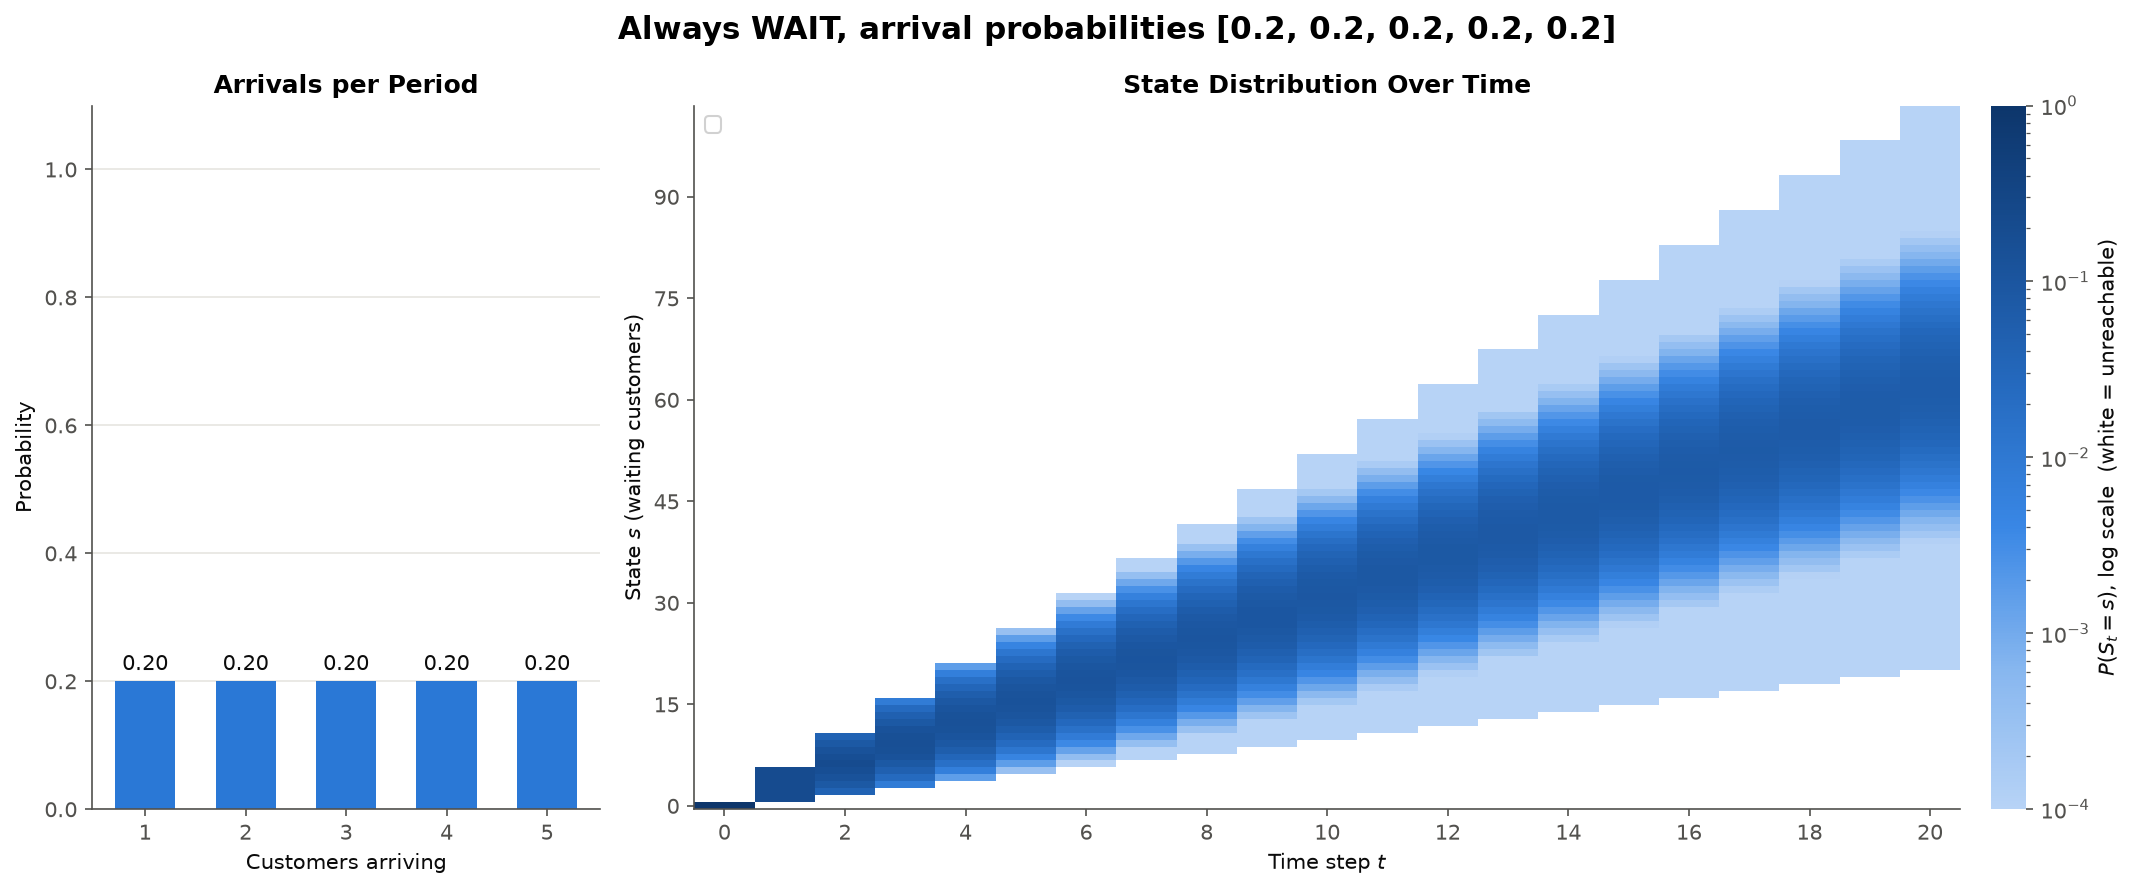
\includegraphics[width=0.49\textwidth]{env_wait_uniform.png}\hfill
  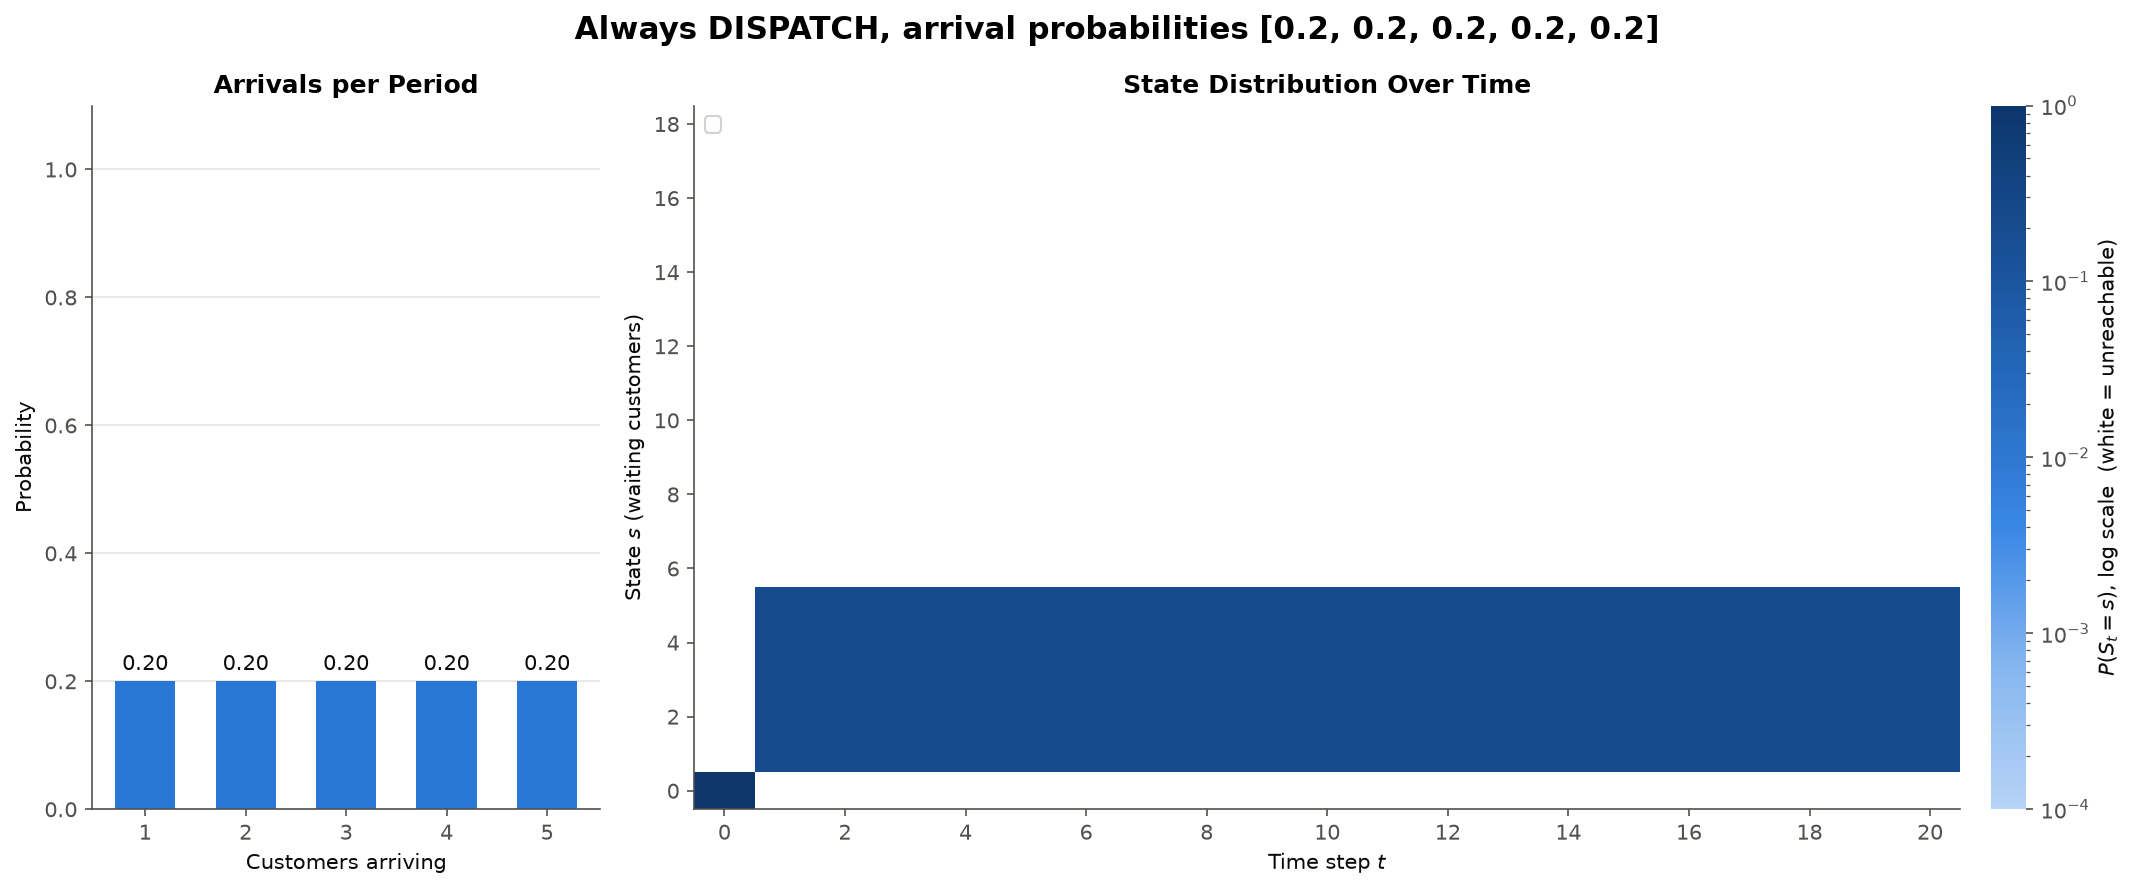
\includegraphics[width=0.49\textwidth]{env_dispatch_uniform.png}
  \caption{Exact state distribution over 20 steps with uniform arrivals, for always \action{Wait} (left) and always \action{Dispatch} (right).}
  \label{fig:env}
\end{figure}

\FloatBarrier
% =====================================================================
\subsection{\texorpdfstring{2a) Enumeration ($T = 500$)}{2a) Enumeration (T = 500)}}

\textbf{Method:} backward induction. Starting from $V_T \equiv 0$, I compute for $t = T-1, \dots, 0$
\[
  V_t(s) = \max_{a}\ \E_{A_t}\big[r(s, a) + V_{t+1}(s')\big],
\]
and the optimal action is the corresponding $\argmax$. The solve takes about 6\,s.

\textbf{Assumptions:}
\begin{itemize}
  \item Initial states $s_0 \in \{0, \dots, 50\}$.
  \item No discounting ($\gamma = 1$): the horizon is finite, so all values are finite anyway. $\gamma = 0.95$ is used in 2b and 2c.
  \item No terminal cost ($V_T \equiv 0$).
  \item No cap at 200 customers: every reachable state is kept (see the edge cases).
\end{itemize}

\subsubsection{\texorpdfstring{Optimal Value Function at $t = 0$}{Optimal Value Function at t = 0}}

\fig{0.72}{2a_value_function.png}{Optimal value function $V_0(s)$ at $t = 0$.}{fig:2a-value}

\begin{itemize}
  \item \textbf{Decreasing in $s$:} more waiting customers always means more future cost. $V_0(0) = -16{,}071.6$, about 32 per period.
  \item \textbf{Flat for $s = 13$--$15$:} here $V_0(s) = V_0(0) - 100$ exactly. The optimal action dispatches, the shuttle takes everyone, and the system is back at an empty queue for the price of one dispatch.
  \item \textbf{Kinks at multiples of $K = 15$:} each further block of 15 customers needs one more shuttle.
\end{itemize}

\subsubsection{Optimal Policy and Simulated Behaviour}

\fig{0.95}{2a_policy_map.png}{Optimal action for every period and queue size.}{fig:2a-policy}

The optimal policy is a \textbf{threshold policy: dispatch if and only if $s \geq 13$}, for $t = 0, \dots, 489$ (Figure~\ref{fig:2a-policy}). Near the end of the horizon:
\begin{itemize}
  \item The threshold briefly drops to 12.
  \item In the last 3 periods, the policy never dispatches. A dispatch removes at most 15 customers and therefore saves at most $3 \cdot 15 \cdot c_h = 90 < c_f = 100$.
\end{itemize}

\fig{0.8}{2a_trajectories.png}{Simulated trajectories under the optimal policy from $s_0 \in \{0, 10, 25, 50\}$.}{fig:2a-traj}

Simulating the policy from $s_0 \in \{0, 10, 25, 50\}$ shows exactly the expected behaviour (Figure~\ref{fig:2a-traj}):
\begin{itemize}
  \item \textbf{Large initial queues are brought down immediately.} From $s_0 = 50$, the policy dispatches in four consecutive periods ($50 \to 39 \to 29 \to 16 \to 4$).
  \item \textbf{Afterwards, all trajectories follow the same sawtooth.} The queue builds up until it reaches 13 and is then emptied.
  \item \textbf{The remaining variation is only due to random arrivals.} Because at most 5 customers arrive per period, the queue at a dispatch is always between 13 and $12 + 5 = 17$ (observed: 13--17, mean 14.3). The time between dispatches ranges from 3 to 8 periods, with a mean of 4.7, which matches $\approx 14.3 / \E[A] = 14.3 / 3$.
  \item \textbf{At the end of the horizon, queues grow unchecked} (16--23 customers at $T$), consistent with the policy map.
\end{itemize}

\subsubsection{Edge Cases}

\begin{center}
\small
\begin{tabularx}{\textwidth}{@{}p{3.6cm}L@{}}
  \toprule
  \textbf{Edge case} & \textbf{Handling} \\
  \midrule
  Fewer than $K$ customers (or none) when dispatching & The remaining queue is $\max(0, s - K)$, so it is never negative. The dispatch still costs $c_f$, so the optimal policy never dispatches an empty station unless $c_f = 0$. \\
  Unbounded queue growth & At most 5 customers arrive per period, so at time $t$ the value table holds all $50 + 5t + 1$ reachable states. Every successor state therefore exists: exact values, no truncation or boundary effects. The 200 cap is never needed, since the optimal policy keeps the queue at 17 or below. \\
  Invalid arrival distribution & An error is raised for mismatched lengths, negative probabilities, or probabilities that do not sum to 1. The sum is compared with a tolerance, so rounding errors such as $5 \times 0.2$ are accepted. \\
  Ties between actions & The solver returns the first maximiser (\action{Dispatch}). Ties only occur in degenerate cases, e.g.\ $c_f = 0$ at $s = 0$. \\
  End of the horizon & $V_T \equiv 0$ makes leftover customers free, so the policy stops dispatching in the last 3 periods. This is a property of the model, not a bug. \\
  \bottomrule
\end{tabularx}
\end{center}

\subsubsection{Tests for Validating Correctness}

All five tests pass.

\textbf{1. Remove the stochasticity.} With exactly 3 arrivals per period, the problem is deterministic, so the optimum is the best of all $2^T$ action sequences. For $T = 12$ (4,096 sequences) and every $s_0 \in \{0, \dots, 30\}$, the DP value equals the brute-force optimum exactly (maximum error 0; Figure~\ref{fig:2a-brute}).

\fig{0.75}{2a_brute_force.png}{Deterministic arrivals: dynamic programming vs.\ brute force over all $2^{12}$ action sequences.}{fig:2a-brute}

\textbf{2. Extreme parameters with obvious answers} ($T = 60$, Figure~\ref{fig:2a-extreme}):

\begin{center}
\begin{tabular}{@{}ll@{}}
  \toprule
  \textbf{Setting} & \textbf{Expected and observed} \\
  \midrule
  $c_h = 0$ & Never dispatch, $V \equiv 0$ \\
  $c_f = 0$, or $c_h = 200 > c_f$ & Dispatch whenever $s \geq 1$ \\
  $K = 0$ & Never dispatch, $V_0(0) = -c_h\,\E[A]\,\frac{T(T-1)}{2} = -10{,}620$ \\
  \bottomrule
\end{tabular}
\end{center}

\fig{1.0}{2a_extreme_cases.png}{Optimal policy in the extreme cases.}{fig:2a-extreme}

\textbf{3. Parameter sweeps.} I changed one parameter at a time and recorded the dispatch threshold at $t = 0$ (Figure~\ref{fig:2a-sweeps}):

\begin{center}
\small
\begin{tabularx}{\textwidth}{@{}llL@{}}
  \toprule
  \textbf{Change} & \textbf{Threshold} & \textbf{Reason} \\
  \midrule
  Dispatch cost $c_f$ $\uparrow$ & Rises, $0 \to 15$ & An expensive shuttle is worth filling up first. \\
  Waiting cost $c_h$ $\uparrow$ & Falls, $15 \to 1$ & Expensive waiting forces earlier dispatches. \\
  Capacity $K$ $\uparrow$ & Rises, then flat at 16 & Once the shuttle is large, capacity stops being the bottleneck. \\
  \bottomrule
\end{tabularx}
\end{center}

\fig{1.0}{2a_parameter_sweeps.png}{Dispatch threshold at $t = 0$ when one parameter is varied at a time.}{fig:2a-sweeps}

The threshold never exceeds $K$, and the policy stays threshold-shaped in all 30 variants.

\textbf{4. First 10 steps.} For one simulated trajectory, I checked at every step that $V_t(s_t) = \max_a Q_t(s_t, a)$, that the action is the $\argmax$, and that the reward matches the formula:

\begin{center}
\small
\setlength{\tabcolsep}{4.5pt}
\begin{tabular}{@{}l*{10}{r}@{}}
  \toprule
  $t$ & 0 & 1 & 2 & 3 & 4 & 5 & 6 & 7 & 8 & 9 \\
  \midrule
  $s_t$ & 0 & 3 & 8 & 9 & \textbf{14} & 2 & 5 & 10 & \textbf{13} & 3 \\
  $Q(\text{D}) - Q(\text{W})$ & $-100.0$ & $-66.9$ & $-25.0$ & $-19.1$ & $\mathbf{+17.7}$ & $-77.2$ & $-48.5$ & $-14.3$ & $\mathbf{+7.2}$ & $-66.9$ \\
  Action & W & W & W & W & \textbf{D} & W & W & W & \textbf{D} & W \\
  Reward & 0 & $-6$ & $-16$ & $-18$ & $-100$ & $-4$ & $-10$ & $-20$ & $-100$ & $-6$ \\
  \bottomrule
\end{tabular}
\end{center}

\fig{0.6}{2a_first_10_steps.png}{First 10 steps of a simulated trajectory: state, advantage of dispatching, and reward.}{fig:2a-first10}

The advantage of dispatching grows as the queue fills up. It turns positive exactly when the threshold of 13 is reached, and the queue is then emptied (Figure~\ref{fig:2a-first10}).

\textbf{5. Optimal vs.\ other policies.} Starting from $s_0 = 0$, I compared $V^*$ with simulated rollouts and with the \emph{exact} expected values (computed by exact policy evaluation) of a random policy and of every fixed threshold rule ``dispatch if $s \geq k$'' (Figure~\ref{fig:2a-random}):

\begin{center}
\begin{tabular}{@{}ll@{}}
  \toprule
  \textbf{Policy} & \textbf{Expected total reward} \\
  \midrule
  \textbf{Optimal, $V^*_0(0)$} & $\mathbf{-16{,}071.6}$ \\
  Optimal, mean of 50 rollouts & $-16{,}120.5$ (sampling noise around $V^*$) \\
  Best fixed threshold, $k = 13$ & $-16{,}099.9$ \\
  Random, dispatching with probability 0.5 & $-28{,}299.9$ (all 50 rollouts below $V^*$) \\
  \bottomrule
\end{tabular}
\end{center}

\fig{1.0}{2a_optimal_vs_random.png}{The optimal policy compared with a random policy and with every fixed threshold rule.}{fig:2a-random}

No other policy beats $V^*$. The best fixed threshold is the one the dynamic program found ($k = 13$); it is slightly worse than $V^*$ only because the optimal policy also adapts near the end of the horizon.

\FloatBarrier
% =====================================================================
\subsection{\texorpdfstring{2b) Value Iteration ($T = \infty$)}{2b) Value Iteration (infinite horizon)}}

\textbf{Method:} starting from $V \equiv 0$, I repeatedly apply the Bellman optimality update to every state $s \in \{0, \dots, 200\}$:
\[
  V(s) \leftarrow \max_{a}\ \E_{A}\big[r(s, a) + \gamma\,V(s')\big].
\]
The values are updated in place, so later states within a sweep already use the new values. I stop when the largest change in a sweep, $\Delta_k = \max_s |V_k(s) - V_{k-1}(s)|$, drops below $10^{-8}$; this takes 343 sweeps. The policy is the greedy $\argmax$ with respect to the final $V$.

\textbf{Assumptions:}
\begin{itemize}
  \item Discount factor $\gamma = 0.95$.
  \item At most 200 customers: a next state above 200 is clamped to 200, i.e.\ extra customers are turned away (see the edge cases).
\end{itemize}

\subsubsection{Optimal Value Function}

\fig{0.95}{2b_value_function.png}{Optimal value function from value iteration.}{fig:2b-value}

\begin{itemize}
  \item \textbf{Decreasing in $s$:} as in 2a, more waiting customers always means more future cost. $V^*(0) = -576.7$, i.e.\ $(1 - \gamma)\,V^*(0) \approx -28.8$ per period. This is lower than the 32 per period of 2a because discounting weights the cheap first periods after starting from an empty station most.
  \item \textbf{Same shape as in 2a:} flat at $s = 13$--$15$, with kinks at multiples of $K = 15$. Tests 1--3 explain these features exactly.
\end{itemize}

\subsubsection{Optimal Policy and Simulated Behaviour}

The optimal policy is again the \textbf{threshold policy: dispatch if and only if $s \geq 13$}. This is the same threshold as in 2a, and it holds for all 201 states.

\fig{0.8}{2b_trajectories.png}{Simulated trajectories under the value-iteration policy.}{fig:2b-traj}

The simulation from 2a, repeated with the value-iteration policy, shows the same behaviour (Figure~\ref{fig:2b-traj}):
\begin{itemize}
  \item Large queues are cleared immediately, then every trajectory follows the ``13 $\to$ dispatch'' sawtooth.
  \item Every dispatch happens at a queue of 13--17 (mean 14.3), with 3--8 periods between dispatches (mean 4.7).
  \item \textbf{Unlike in 2a, there is no end-of-horizon effect.} The policy does not depend on time, so the queue stays at 17 or below until $t = 500$ and beyond. This confirms that the behaviour at the end of 2a came from the finite horizon.
\end{itemize}

\subsubsection{Edge Cases}

The edge cases of the shared environment (dispatching fewer than $K$ customers, invalid arrival distributions) are handled as described in 2a.

\begin{center}
\small
\begin{tabularx}{\textwidth}{@{}p{3.6cm}L@{}}
  \toprule
  \textbf{Edge case} & \textbf{Handling} \\
  \midrule
  Next state above the cap of 200 & The value of $\min(s', 200)$ is used: the queue cannot exceed 200, and extra customers are turned away. Doubling the cap to 400 leaves $V^*$ on $s \leq 50$ unchanged (difference exactly 0), so the cap does not affect the states that occur. \\
  Invalid discount factor & Value iteration only converges for $0 \leq \gamma < 1$ (with $\gamma = 1$ the infinite sum of costs diverges). Any other value raises an error; tested for $\gamma = 1$, $1.5$ and $-0.1$. \\
  When to stop & There is no fixed number of sweeps. The solver stops at $\Delta_k < 10^{-8}$. \\
  Initial values & $V \equiv 0$. Any starting point converges to the same $V^*$; starting from 0 makes sweep $k$ comparable to a $k$-period enumeration (Test 6). \\
  Ties between actions & As in 2a: the solver returns \action{Dispatch} on a tie, which only happens in degenerate cases. \\
  \bottomrule
\end{tabularx}
\end{center}

\subsubsection{Tests for Validating Correctness}

All tests pass. Tests 1--3 check that the structure of $V^*$ matches what the model predicts, Tests 4--5 check the iteration itself, and Test 6 compares against an independent method.

\textbf{1. What does one more customer cost?} $V^*(s) - V^*(s-1)$ is the value of one extra waiting customer (Figure~\ref{fig:2b-marginal}).
\begin{itemize}
  \item It is never positive, and it shrinks as the queue approaches the threshold, because a shuttle is coming soon.
  \item It is \textbf{exactly 0 for $s = 14, 15$:} at $s \geq 13$ the policy dispatches anyway, and up to $K = 15$ everyone fits in, so an extra customer just rides along.
  \item At $s = 16$ it jumps back to $-10.77$, exactly the cost of the very first customer: the 16th customer is left behind alone.
\end{itemize}

\fig{0.6}{2b_marginal_cost.png}{Cost of one more waiting customer, $V^*(s) - V^*(s-1)$.}{fig:2b-marginal}

\textbf{2. Where does \action{Dispatch} take over from \action{Wait}?} For every $s \leq K$, a dispatch takes everyone, so the system afterwards is exactly where an empty station would be after waiting:
\[
  Q(s, \action{Dispatch}) = -c_f + \gamma\,\E[V^*(A)] = V^*(0) - c_f = -676.67 \qquad \text{for all } s \leq K.
\]
$Q(s, \action{Wait})$ decreases with every customer and drops below this constant floor at $s = 13$, the threshold (Figure~\ref{fig:2b-q}). This also matches 2a.

\fig{0.95}{2b_q_values.png}{Q-values of both actions and the switch from \action{Wait} to \action{Dispatch}.}{fig:2b-q}

\textbf{3. The value function repeats every $K = 15$ customers.} Dispatching turns $s$ customers into $s - K$ for a price of $c_f$. If the $s - K$ customers left behind are below the threshold, then $V^*(s) = V^*(s - K) - c_f$ exactly (Figure~\ref{fig:2b-period}).
\begin{itemize}
  \item This holds exactly for $s = 15$--$27$.
  \item From $s = 28$ on, the customers left behind are themselves at the threshold and need their own shuttle soon, so the gap grows beyond 100.
\end{itemize}

\fig{0.6}{2b_periodicity.png}{The value function repeats every $K$ customers.}{fig:2b-period}

\textbf{4. Convergence.} The Bellman update is a $\gamma$-contraction, so $\Delta_k$ must decay at least as fast as $\gamma^k$, which is a straight line on a log scale (Figure~\ref{fig:2b-conv}).
\begin{itemize}
  \item After a short initial phase, $\Delta_k$ shrinks by a factor of 0.937 per sweep (median over the last 100 sweeps).
  \item This is slightly faster than $\gamma = 0.95$ because of the in-place updates.
\end{itemize}

\fig{0.75}{2b_convergence.png}{Convergence of value iteration: largest change per sweep.}{fig:2b-conv}

\textbf{5. How the Q-values and the policy evolve.} After every sweep $k$, the current $V_k$ defines a greedy policy. Figure~\ref{fig:2b-heatmap} shows $Q_k(\action{Dispatch}) - Q_k(\action{Wait})$ for every sweep and state:
\begin{itemize}
  \item \textbf{Sweeps 1--2:} $V \approx 0$ ignores the future, and waiting (at most $2 \cdot 15 = 30$ per period) looks cheaper than a dispatch (100), so the policy never dispatches.
  \item \textbf{Sweeps 3--34:} the threshold jumps to 14, overshoots down to 10, and then climbs back via 11 and 12.
  \item \textbf{From sweep 35 of 343:} the policy is final at 13, although the values are still up to 77 away from $V^*$. Only the sign of the advantage matters for the action, which is exactly what policy iteration (2c) exploits.
\end{itemize}

\fig{0.6}{2b_q_heatmap.png}{Advantage of dispatching over the sweeps of value iteration.}{fig:2b-heatmap}

\textbf{6. Cross-check with enumeration (2a).} I ran the enumeration solver from 2a with the same $\gamma = 0.95$. Its value for horizon $n$, $V_0^{(n)}$, should approach $V^*$ like $\gamma^n$, since backward induction from $V \equiv 0$ is value iteration started from 0 (Figure~\ref{fig:2b-cross}).
\begin{itemize}
  \item The gap stays below $\gamma^n \cdot$ (initial gap) for every horizon $n$, reaching $1.4 \cdot 10^{-4}$ at $n = 300$.
  \item Both solvers choose the same action in every state $s \leq 50$.
\end{itemize}

\fig{1.0}{2b_enumeration_crosscheck.png}{Discounted enumeration converges to $V^*$.}{fig:2b-cross}

\FloatBarrier
% =====================================================================
\subsection{2c) Policy Iteration}

\textbf{Method:} starting from the policy $\pi_0$ = ``always wait'', I alternate two steps until the policy no longer changes:
\begin{enumerate}
  \item \textbf{Policy evaluation:} repeat $V(s) \leftarrow \E_{A}\big[r(s, \pi(s)) + \gamma\,V(s')\big]$ for all states until the largest change is below $\theta = 10^{-6}$. Each evaluation starts from the values of the previous policy (warm start).
  \item \textbf{Policy improvement:} set $\pi(s) \leftarrow \argmax_a \E_A\big[r(s, a) + \gamma\,V(s')\big]$. An action is only switched if the new one is better by more than the evaluation error $\gamma\theta/(1-\gamma) = 1.9 \cdot 10^{-5}$.
\end{enumerate}
This converges after \textbf{6 policy evaluations}.

\textbf{Assumptions:} as in 2b ($\gamma = 0.95$, next states clamped at 200), plus the evaluation tolerance $\theta = 10^{-6}$ and the initial policy ``always wait''.

\subsubsection{Optimal Policy}

\fig{0.95}{2c_policy.png}{Optimal policy from policy iteration.}{fig:2c-policy}

The optimal policy is the \textbf{threshold policy: dispatch if and only if $s \geq 13$} (Figure~\ref{fig:2c-policy}). It is identical to value iteration in all 201 states and to the steady-state policy of enumeration. The value function also matches 2b (maximum difference $1.9 \cdot 10^{-5}$), so it is not shown again.

\subsubsection{Edge Cases}

The edge cases of the environment (2a) and of the state cap (2b) apply unchanged; doubling the cap to 400 again leaves policy and values on $s \leq 50$ unchanged.

\begin{center}
\small
\begin{tabularx}{\textwidth}{@{}p{3.6cm}L@{}}
  \toprule
  \textbf{Edge case} & \textbf{Handling} \\
  \midrule
  Ties and evaluation noise & Policy evaluation is only accurate up to $\gamma\theta/(1-\gamma)$. If the solver switched to any action that looks marginally better, two (nearly) equally good actions could swap back and forth forever. It therefore switches only for an improvement larger than this error. Test: with $c_f = c_h = 0$, every Q-value is 0, and the solver keeps its initial policy and stops after one evaluation. \\
  Termination & Policy iteration terminates in theory, since there are finitely many policies and each iteration strictly improves. As a safeguard, a maximum number of iterations (default 100) raises an error instead of looping forever; tested with a limit of 2. \\
  Inaccurate policy evaluation & Evaluation stops at $\Delta < \theta$. I checked the result against an exact linear solve (Test 3), and every check that compares values allows for this error. \\
  Initial policy & Any policy can be passed in. One that does not cover every state raises an error. The result does not depend on it (Test 4). \\
  Initial policy ``always wait'' & This policy never empties the station, so its value depends on the cap: at $s = 200$ it pays $c_h \cdot 200$ forever, $V^{\pi_0}(200) = -2 \cdot 200 / (1 - \gamma) = -8{,}000$ exactly. The clamp keeps this finite and well-defined. \\
  Invalid discount factor & As in 2b, $\gamma \notin [0, 1)$ raises an error. \\
  \bottomrule
\end{tabularx}
\end{center}

\subsubsection{Tests for Validating Correctness}

All four tests pass.

\textbf{1. How the policy evolves.} Each row of Figure~\ref{fig:2c-evolution} shows the policy evaluated in one iteration:

\begin{center}
\begin{tabular}{@{}l*{6}{r}@{}}
  \toprule
  \textbf{Iteration} & 0 & 1 & 2 & 3 & 4 & 5 \\
  \midrule
  First state with \action{Dispatch} & never & 3 & 26 & 7 & 14 & \textbf{13} \\
  $V^{\pi_k}(0)$ & $-2{,}204$ & $-1{,}330$ & $-891$ & $-749$ & $-582$ & $\mathbf{-577}$ \\
  \bottomrule
\end{tabular}
\end{center}

\fig{0.9}{2c_policy_evolution.png}{Policy after each iteration of policy iteration.}{fig:2c-evolution}

\begin{itemize}
  \item \textbf{$\pi_1$ dispatches almost always.} Under ``always wait'', the queue grows forever, so $V^{\pi_0}$ is very low and dispatching looks attractive almost everywhere.
  \item \textbf{Intermediate policies need not be thresholds.} $\pi_2$ dispatches at 26--29, waits at 30--32, and dispatches again from 33, because it acts greedily on the values of a bad policy.
  \item \textbf{The policy settles in a few steps.} It narrows down to 14 and then to 13. Every iteration except the last changes the policy.
\end{itemize}

\textbf{2. Policy improvement theorem.} Acting greedily on $V^{\pi_k}$ can never make things worse, so $V^{\pi_{k+1}}(s) \geq V^{\pi_k}(s)$ must hold for every state and iteration (Figure~\ref{fig:2c-improvement}).
\begin{itemize}
  \item The smallest improvement over all states per iteration is $+160$, $+110$, $+79$ and $+2.5$.
  \item The first step shows $-1.8 \cdot 10^{-5}$ at $s = 199$, where both policies wait. This is within the evaluation error.
  \item The value curves end on $V^*$ from value iteration.
\end{itemize}

\fig{1.0}{2c_policy_improvement.png}{Value of each policy during policy iteration.}{fig:2c-improvement}

\textbf{3. Agreement with exact evaluation and value iteration.} For a fixed policy, the Bellman equation is linear, so $V^\pi$ can also be computed exactly by solving $(I - \gamma P_\pi)\,V = r_\pi$ (a $201 \times 201$ system; Figure~\ref{fig:2c-agreement}).
\begin{itemize}
  \item Policy iteration chooses the same action as value iteration in all 201 states.
  \item Its values differ from the exact solution by at most $1.86 \cdot 10^{-5}$ and from value iteration by at most $1.87 \cdot 10^{-5}$. Both are below the evaluation error bound of $1.9 \cdot 10^{-5}$.
  \item \textbf{Effort:} policy iteration needs only 6 policies, but evaluating them iteratively costs 1,930 sweeps in total, compared with 343 sweeps for value iteration. Each iterative evaluation is itself a value-iteration-like process to tolerance $\theta$, and the values change a lot between policies, so the warm start helps little. The small number of improvement steps would only pay off with cheaper evaluation, e.g.\ one exact linear solve per policy, or a looser $\theta$ in early iterations.
\end{itemize}

\fig{1.0}{2c_agreement_and_effort.png}{Agreement with exact evaluation and value iteration, and computational effort.}{fig:2c-agreement}

\textbf{4. Independence of the initial policy.} The optimal policy is unique, so every starting point must lead to it (Figure~\ref{fig:2c-initial}):

\begin{center}
\small
\begin{tabular}{@{}lrrl@{}}
  \toprule
  \thead[l]{Initial policy} & \thead[r]{Evalu-\\ations} & \thead[r]{Evaluation\\sweeps} & \thead[l]{First state with \action{Dispatch}\\per iteration} \\
  \midrule
  Always wait (default) & 6 & 1,930 & never $\to$ 3 $\to$ 26 $\to$ 7 $\to$ 14 $\to$ 13 \\
  Always dispatch & 5 & 1,600 & 0 $\to$ 45 $\to$ 5 $\to$ 14 $\to$ 13 \\
  Dispatch if $s \geq 1$ & 5 & 1,600 & 1 $\to$ 45 $\to$ 5 $\to$ 14 $\to$ 13 \\
  Dispatch if $s \geq 30$ & 4 & 1,231 & 30 $\to$ 7 $\to$ 14 $\to$ 13 \\
  Random (each state 50/50) & 4 & 1,236 & 1 $\to$ 17 $\to$ 11 $\to$ 13 \\
  \bottomrule
\end{tabular}
\end{center}

\fig{0.75}{2c_initial_policies.png}{Policy iteration from different initial policies.}{fig:2c-initial}

All five runs end in exactly the policy from value iteration after at most 6 evaluations.

\FloatBarrier
\begin{summarybox}{Summary of Part 2}
\begin{tabularx}{\linewidth}{@{}lLLL@{}}
  \toprule
  & \textbf{Enumeration (2a)} & \textbf{Value iteration (2b)} & \textbf{Policy iteration (2c)} \\
  \midrule
  Horizon, discount & $T = 500$, $\gamma = 1$ & $\infty$, $\gamma = 0.95$ & $\infty$, $\gamma = 0.95$ \\
  Optimal policy & Dispatch if $s \geq 13$ (except the last $\sim$10 periods) & Dispatch if $s \geq 13$ & Dispatch if $s \geq 13$ \\
  Work until done & 1 backward pass, 500 steps & 343 sweeps (policy final after 35) & 6 policies, 1,930 evaluation sweeps \\
  \bottomrule
\end{tabularx}

\medskip
All three methods agree on the same threshold policy. The tests confirm it in different ways: brute force, closed-form properties of $V^*$, convergence theory, and exact policy evaluation.
\end{summarybox}

% =====================================================================
\subsection{Given an Additional 3 Months, What Other Validation Tests and Experiments Would I Perform?}

The problem is small (201 states, 2 actions), and three independent methods already agree, so 3 months is more than this instance needs. I would use the time to check whether the results hold \textbf{beyond this instance} and whether the \textbf{model assumptions} are right:
\begin{itemize}
  \item \textbf{Random problem instances:} run all three solvers on thousands of random parameter sets ($K$, $c_f$, $c_h$, arrival distributions) and automatically check the invariants from this report: the solvers agree, the policy is a threshold policy, $V^*$ decreases in $s$, and brute force matches on small instances.
  \item \textbf{Discount factor towards 1:} $(1-\gamma)\,V^*(0)$ should approach the long-run average cost of about 32 per period found by enumeration in 2a. This would connect the finite-horizon and the discounted results.
  \item \textbf{Cheaper policy evaluation:} replace the iterative evaluation in 2c, which dominated the runtime, with an exact linear solve per policy. Then compare runtimes on larger state spaces.
  \item \textbf{Stress the model:}
  \begin{itemize}
    \item High load ($\E[A] > K$), where the cap of 200 actually binds.
    \item Time-varying (rush-hour) arrivals, where the threshold should change over the day.
    \item A policy tuned for the wrong arrival distribution, to see how much reward it loses.
  \end{itemize}
  \item \textbf{Benchmark for learning algorithms:} since the exact optimum is known, check whether model-free methods (Q-learning, policy gradient) learn the threshold of 13 from simulation alone.
\end{itemize}
